\section{Funktionsweise}
\subsection{Grundprinzip der Probenverdünnung}
Um eine Verdünnung von bis zu 1000-fach zu erreichen, nutzt der Probenverdünner das Prinzip der seriellen Verdünnung, bei dem eine konzentrierte Probe schrittweise mit einem Verdünnungsmittel gemischt wird, um die gewünschte Endkonzentration zu erreichen. Dabei werden präzise Mengen der Probe und des Verdünnungsmittels dosiert und in den nächsten Falcontube zusammengeführt. Bei einer Verdünnung bis 10-fach wird direkt aus der Stammlösung entnommen und in die Zielprobe gegeben. Für höhere Verdünnungen wird die Probe in mehreren Schritten verdünnt, wobei jede Stufe eine weitere Verdünnung darstellt. Die zweite Reihe kann bis zu 100-fach verdünnen, indem sie die erste verdünnte Probe weiter verarbeitet. Die dritte Reihe ermöglicht schließlich eine Verdünnung bis zu 1000-fach, indem sie die bereits verdünnte Probe erneut weiter verdünnt. Auch ist es möglich, dass alle Reihen die diesselbe Verdünnung erreichen, solange genug Stammlösung dafür vorhanden ist. Ebefalls können auch zwei Reihen dasselbe Verdünnungsverhältnis haben und die dritte ein unterschiedlichen. Verdünnungsverhältnisse, die nicht erreicht werden können, werden von der Software blockiert, um eine fehlerhafte Probenvorbereitung zu vermeiden.
\newpage
\subsection{Ablauf eines Verdünnungsvorgangs}
\begin{figure}[h!]
    \centering
    \includegraphics[width=1\textwidth]{Flussdiagramm_Probenverdünner.drawio.png}
    \caption{Ablaufdiagramm}
    \label{fig:Ablaufdiagramm}
\end{figure}






Anhand des Ablaufdiagramms in \autoref{fig:Ablaufdiagramm} wird der generelle Ablauf eines Verdünnungsvorgangs beschrieben. Zunächst muss der Falcontubeständer, die Schottflasche ggf. der Abfall- und der Reinigungsbehälter platziert werden, wie in \autoref{fig:Hubpositionierung}, \autoref{fig:Schottflaschepositionierung} und \autoref{fig:Falcontubespositionierung} zu sehen. 

\begin{figure}[H]
    \centering
    \begin{minipage}[t]{0.6\textwidth}
        \centering
        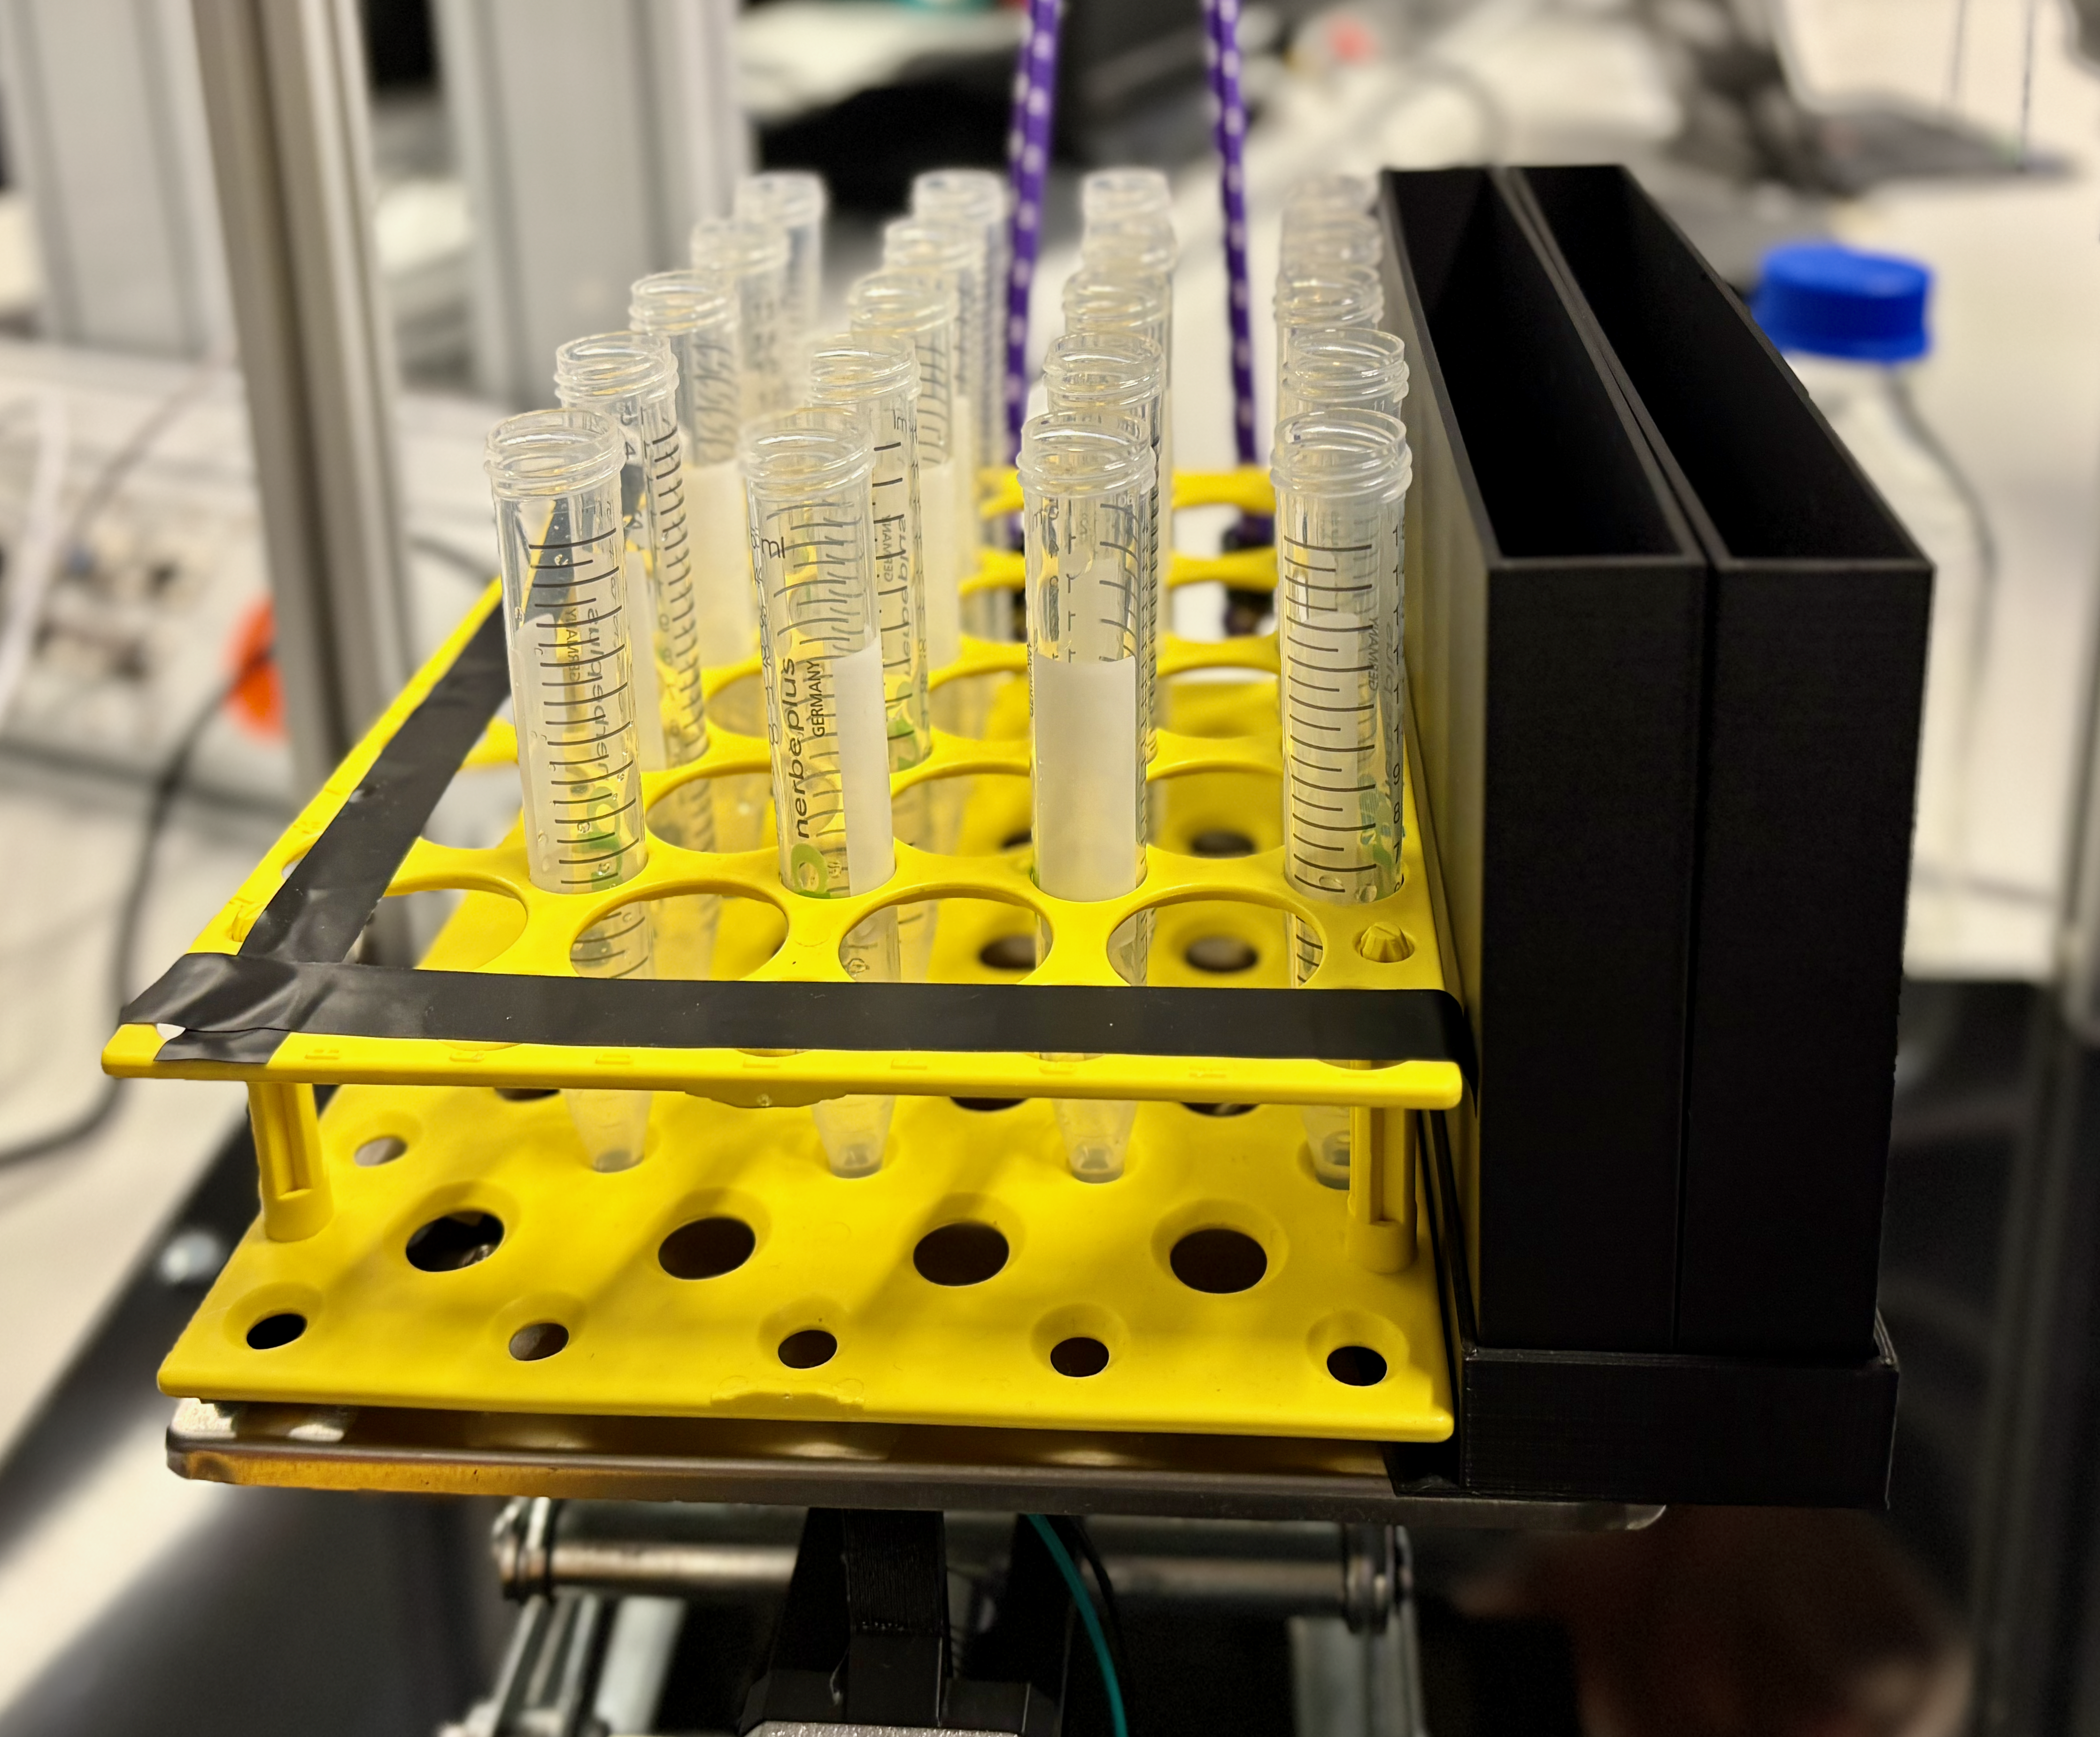
\includegraphics[width=\textwidth]{aufbauaufHubtisch.png}
        \caption{Positionierung der Komponenten auf dem Hubtisch}
        \label{fig:Hubpositionierung}
    \end{minipage}\hfill
    \begin{minipage}[t]{0.35\textwidth}
        \centering
        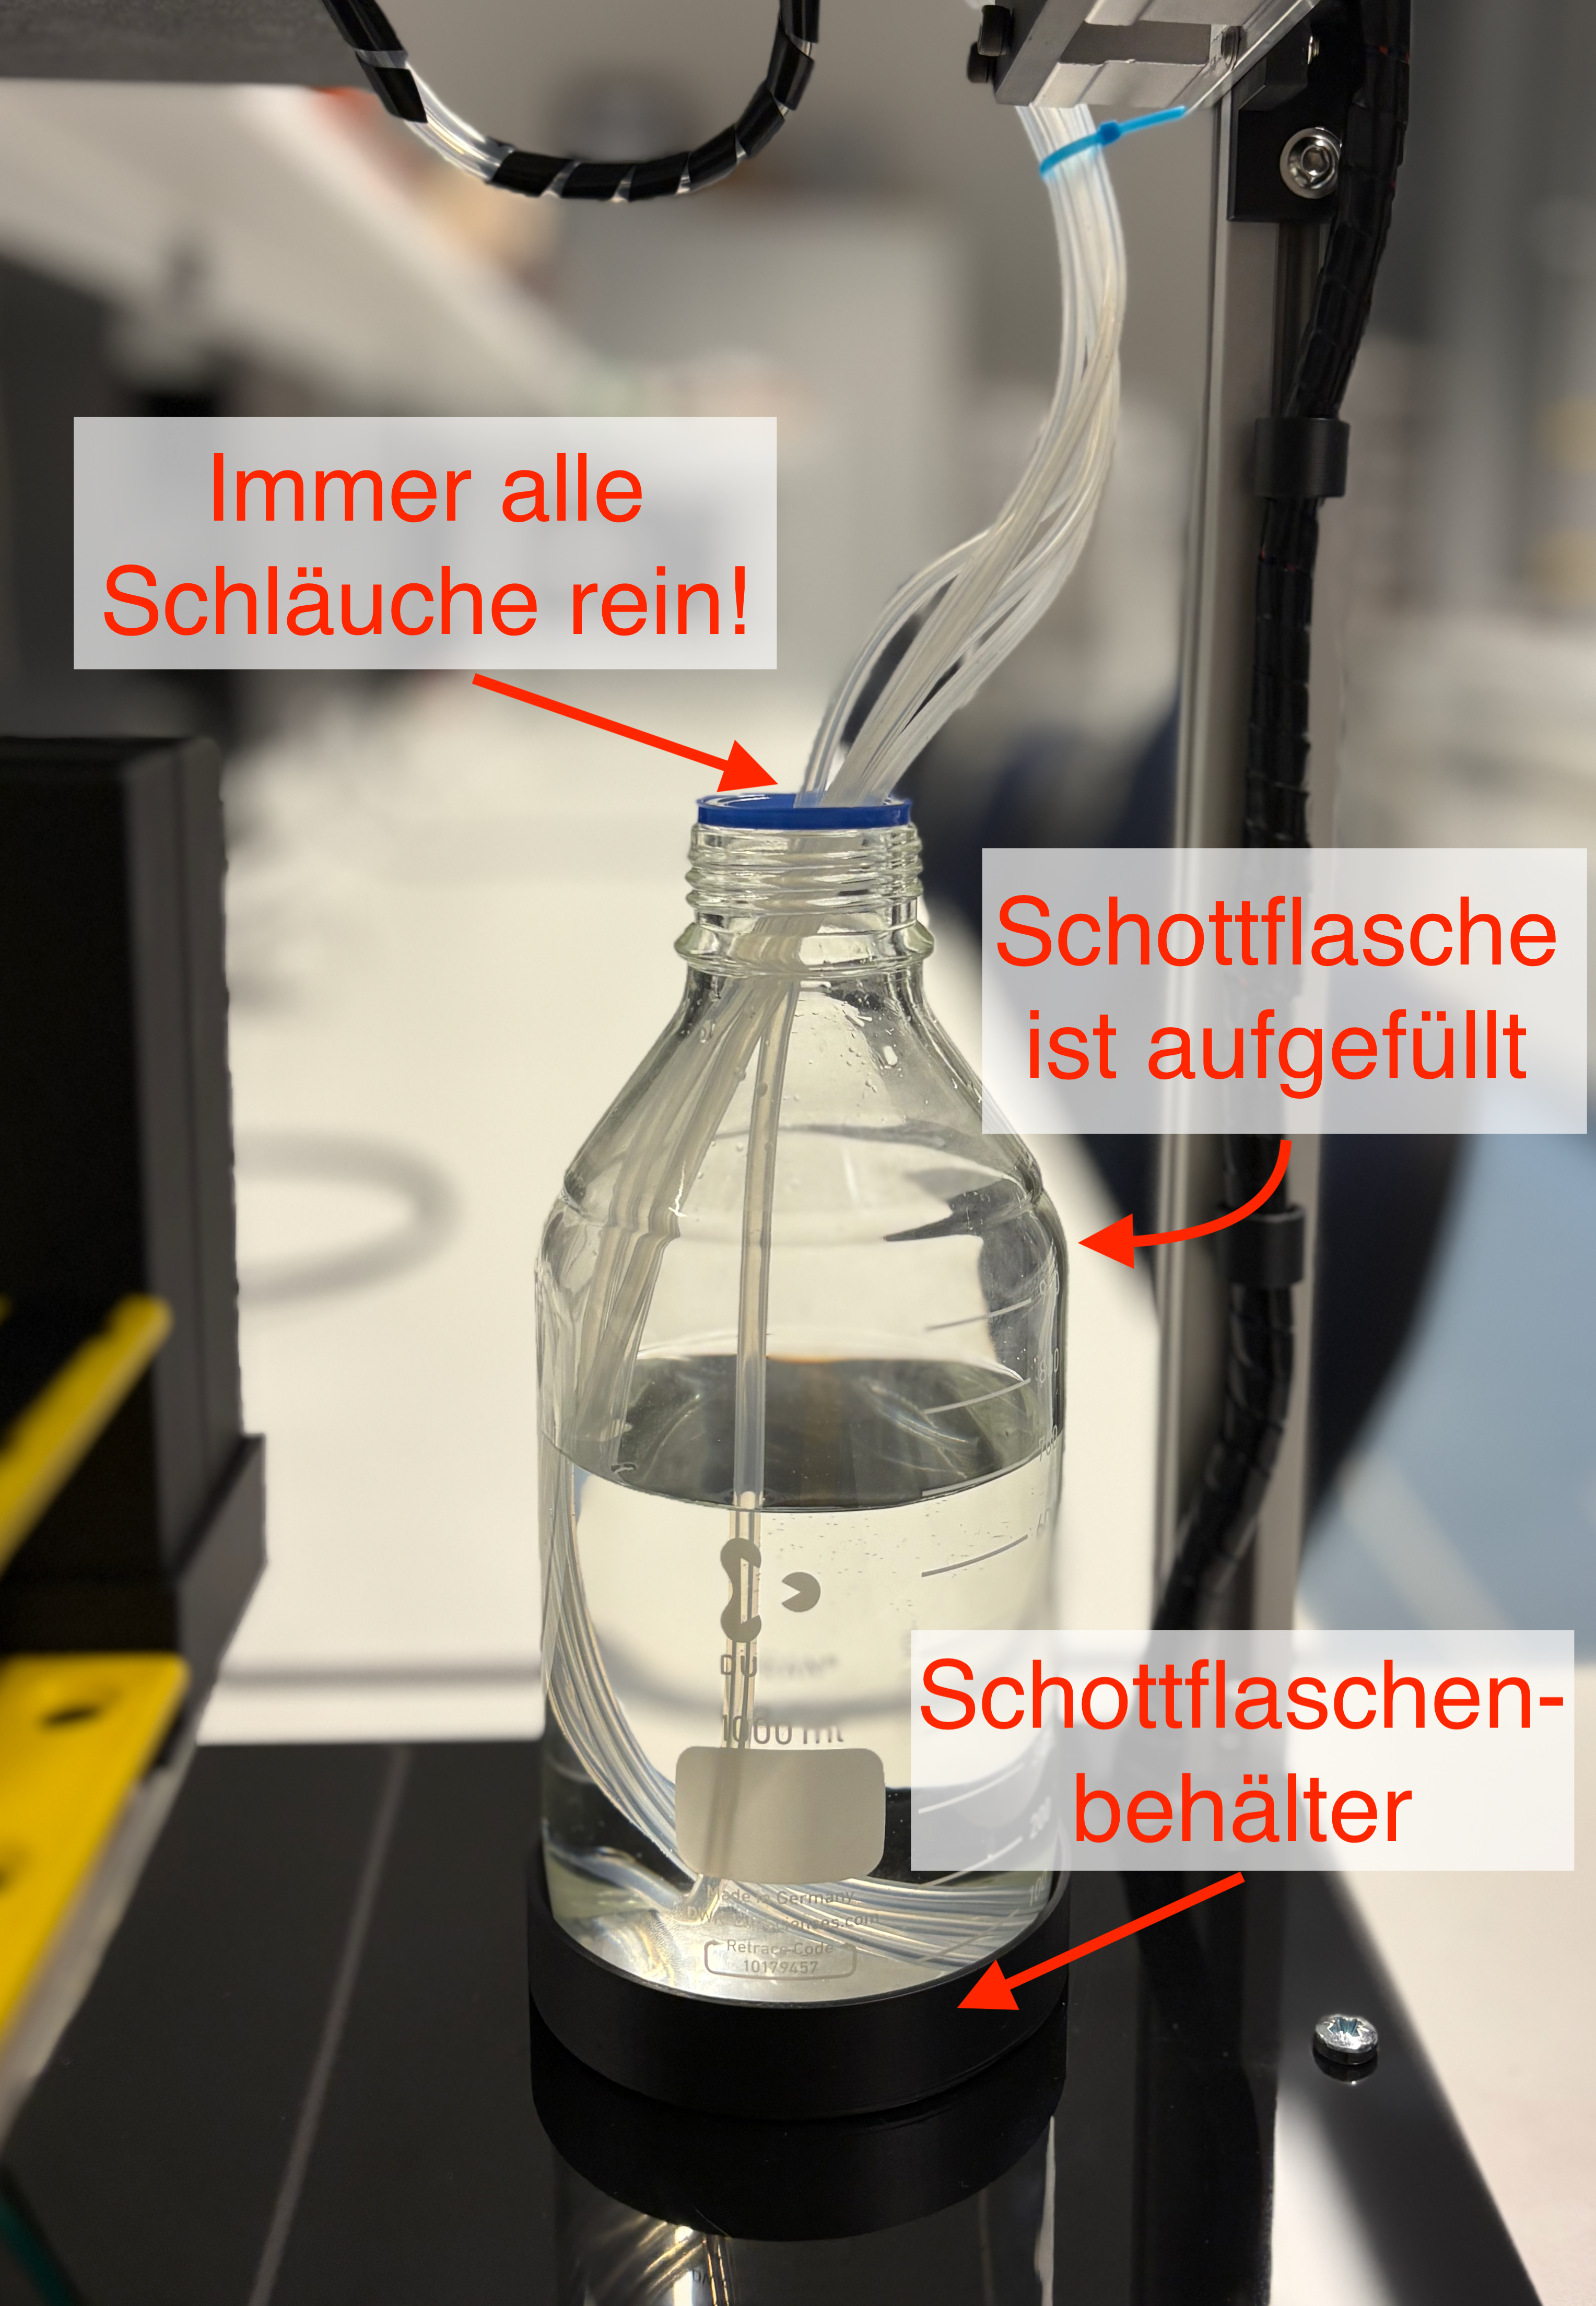
\includegraphics[width=\textwidth]{schottflasche.png}
        \caption{Positionierung der Schottflasche}
        \label{fig:Schottflaschepositionierung}
    \end{minipage}\hfill
\end{figure}

\begin{figure}[H]
    \centering
    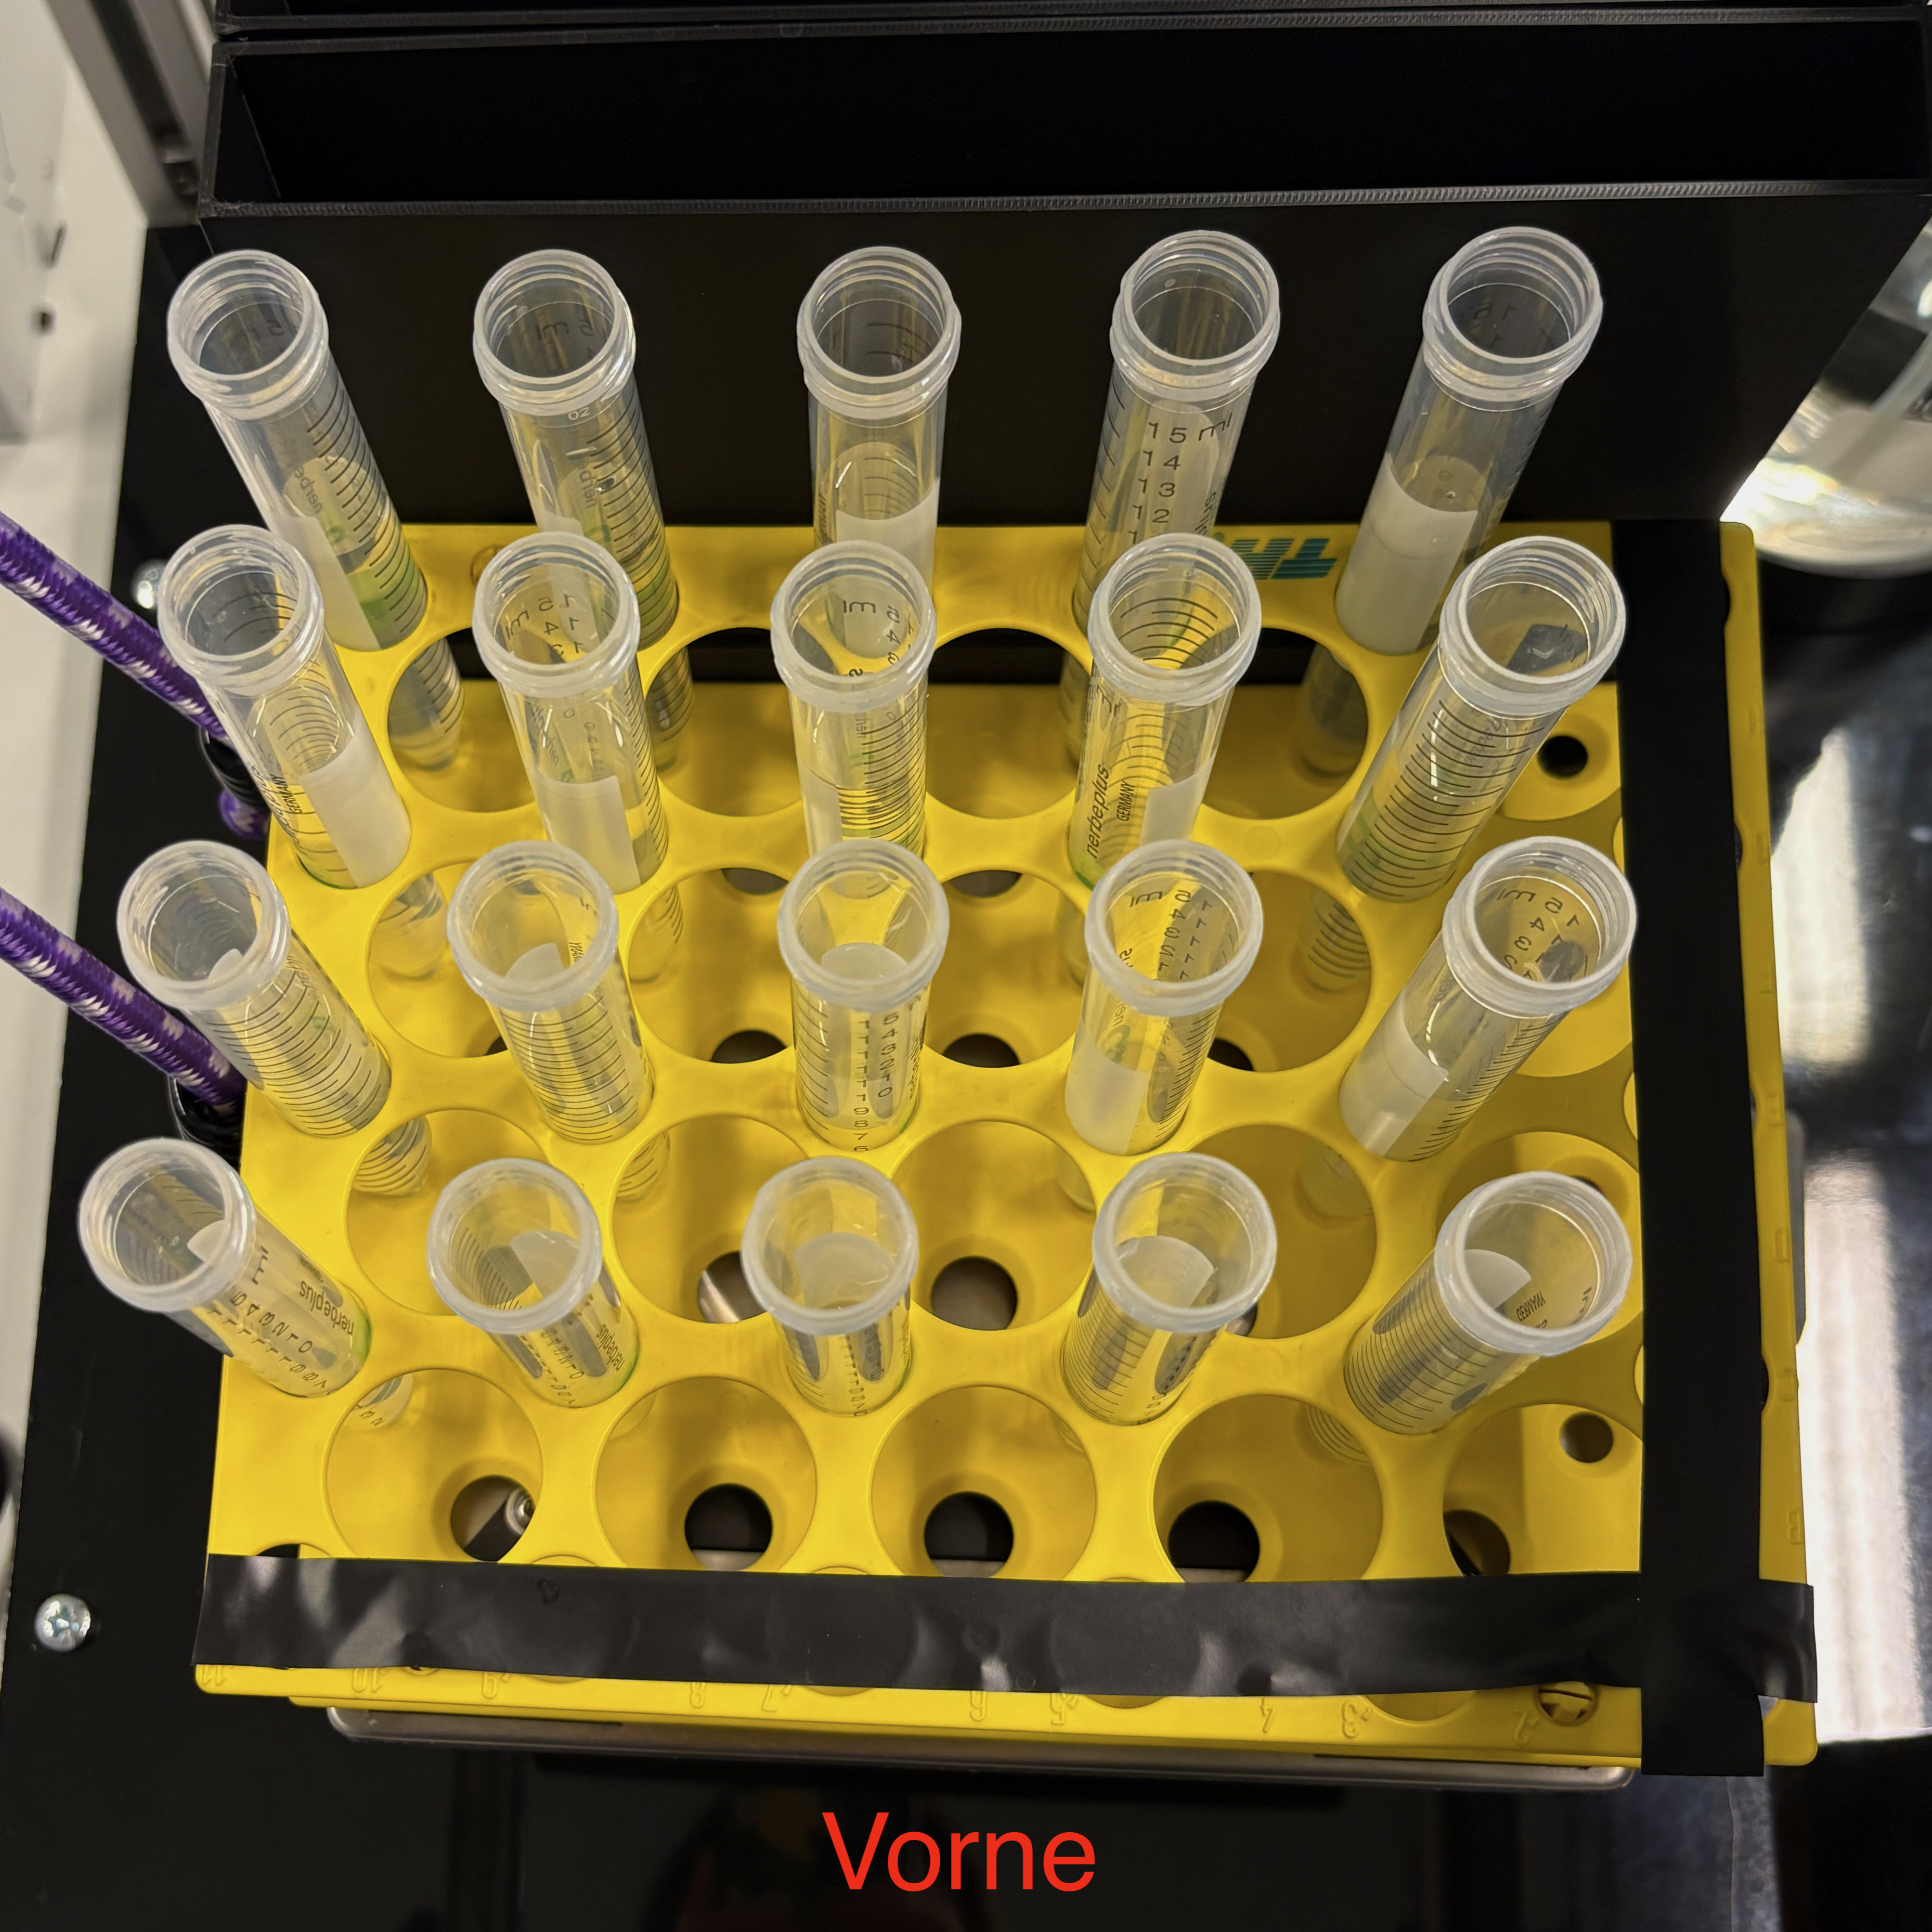
\includegraphics[width=0.6\textwidth]{falconTop.png}
    \caption{Positionierung der Falcontubes}
    \label{fig:Falcontubespositionierung}
\end{figure}



\begin{figure}[h!]
    \centering
    \includegraphics[width=0.8\textwidth]{homepage.png}
    \caption{GUI Startseite zur Eingabe der Verdünnungsparameter}
    \label{fig:GUIerklaerung}
\end{figure}

Danach werden die benötigten Daten in der grafischen Oberfläche eingegeben. Dazu gehört die "Probenspalten"- und "Probenreihen"-Auswahl, das gewünschte Verdünnungsverhältnis für jede Probe, sowie die Volumina der Stammlösung und des Endvolumens, siehe \autoref{fig:GUIerklaerung}. 

Nach der Eingabe der Daten und der Platzierung der Probenbehälter im Gerät, wird der Verdünnungsvorgang gestartet. Das System fährt zunächst die Startposition an und führt eine initiale Reinigung mit der Verdünnungslösung durch, um sicherzustellen, dass alle Schläuche und Spritzen frei von Verunreinigungen sind. 

Daraufhin findet die Zwischenreiningung statt, indem die Spritzen die zu verdünnende Lösung plus 0.5 ml aufziehen und in den Abfallbehälter entsorgen. Anschließend beginnt der eigentliche Verdünnungsschritt, bei dem die Proben entsprechend den eingegebenen Daten verdünnt werden. 

Während des Prozesses werden auch zwischendurch Reinigungsschritte durchgeführt, um Kreuzkontaminationen zu vermeiden. Dieser Vorgang wird wiederholt, bis die letzte Verdünnung erreicht wurde. 

Am Ende des Verdünnungsvorgangs erfolgt eine Entleerung, bei der alle Schläuche in die entgegesetze Pumprichtung Luft aufziehen. 

Optional wird der Falcontubeständer abgedeckt, um die Proben vor der Verdünstung zu schützen. 

Falls die Abdeckung nicht erfolgt, fährt der Spritzenkopf nach hinten in seine Anfangsposition und die Proben können manuell entnommen werden. 

Sollten die Falcuntubes abgedeckt worden sein, muss auf der Website der Abdeckungsentfernen-Vorgang gestartet werden, siehe \autoref{fig:GUIabdeckungentfernen}, bevor die Proben entnommen werden können.

\begin{figure}[H]
    \centering
    \includegraphics[width=0.7\textwidth]{abdeckungentfernen.png}
    \caption{GUI Abdeckungsentfernen Seite}
    \label{fig:GUIabdeckungentfernen}
\end{figure}

Zuletzt sollten der Abfall- und der Reinigungsbehälter geleert werden, um das Gerät für den nächsten Einsatz vorzubereiten.

Wurde der Prozess durch den Not-Aus unterbrochen, muss das System zunächst durch Drücken des Reset-Buttons in der grafischen Oberfläche zurückgesetzt werden, siehe \autoref{fig:start}. Danach kann der Ablauf von Anfang an durchgeführt werden.\\

\newpage
Im folgenden werden noch Ablaufdiagramme der Initialreinigung, der Zwischenreinigung und des Verdünnungsvorgangs dargestellt. Dabei ist die Reihe i, wo die Probenverdünnung stattfinden soll, und die Position wie im Code bestimmt, genauer:
\begin{itemize}
    \item \textbf{Position 1:} Abdeckungsposition
    \item \textbf{Position 2:} Reihe 1 (Stammlösung)
    \item \textbf{Position 3:} Reihe 2
    \item \textbf{Position 4:} Reihe 3
    \item \textbf{Position 5:} Reihe 4
    \item \textbf{Position 6:} Abfallbehälter
    \item \textbf{Position 7:} Reinigungsbehälter
    \item \textbf{Position 8:} Startposition (Home-Position)
\end{itemize}

\FloatBarrier
\begin{figure}[h!]
    \vspace{10mm}
    \centering
    \includegraphics[width=1\textwidth]{Reinigungsprozess_Anfang.drawio.png}
    \caption{Ablaufdiagramm der Initialreinigung}
    \label{fig:AblaufdiagrammInitialreinigung}
\end{figure}

\begin{figure}[h!]
    \vspace{10mm}
    \centering
    \includegraphics[width=1\textwidth]{Reinigungsprozess_Probenentnahme.drawio.png}
    \caption{Ablaufdiagramm der Zwischenreinigung}
    \label{fig:AblaufdiagrammZwischenreinigung}
\end{figure}

\begin{figure}[h!]
    \vspace{10mm}
    \centering
    \includegraphics[width=0.7\textwidth]{Verdünnungsschritt.drawio.png}
    \caption{Ablaufdiagramm des Verdünnungsvorgangs}
    \label{fig:AblaufdiagrammVerdünnungsvorgang}
\end{figure}

\FloatBarrier

